\exerciseappendix

\begin{enumerate}
\def\labelenumi{\arabic{enumi})}
\tightlist
\item
  Let E be a Hausdorff locally convex space, K a compact convex subset of E, and S a set of continuous affine linear transformations from K into itself, which is stable under composition. The set S is said to be distal if, for every pair of distinct points \(a\) , \(b\) in K, the closure of the set of pairs \((s.a,s.b)\) , where \(s\) ranges over S, does not contain any point of the diagonal of \(\mathbf{K} \times \mathbf{K}\) . a) Show that an equicontinuous group of affine transformations of K is distal.
\end{enumerate}

\begin{enumerate}
\def\labelenumi{\alph{enumi})}
\setcounter{enumi}{1}
\tightlist
\item
  Show that if K is non-empty and S is distal, then there exists at least one point of K which is invariant under every transformation of S. (If M is a non-empty compact convex subset of K which is stable under S, show that if M contains two distinct points \(x_{1}, x_{2}\) , and if A is the closure of the orbit of \(x = \frac{x_{1} + x_{2}}{2}\) , then A cannot contain any extremal point of M. Deduce that if L is a minimal element of the family of non-empty compact convex subsets of K, which are stable under S, then L reduces to a point; argue by reductio ad absurdum: with the same notations, the closed convex envelope of A would be equal to L, which would contradict the Krein-Milman theorem.)
\end{enumerate}

\begin{enumerate}
\def\labelenumi{\arabic{enumi})}
\setcounter{enumi}{1}
\tightlist
\item
  Let E be a Banach space, K a precompact subset of E which is not a single point, and d the diameter of K. Show that there exists a point \(x_{0} \in K\) and a number r such that 0 \textless{} r \textless{} d, such that \(\|x - x_{0}\| \leqslant r\) for all \(x \in K\) (choose \(\varepsilon > 0\) small enough, and n points \(y_{1}, \ldots, y_{n}\) of K such that every point of K is at a distance \(<\varepsilon\) from one of the \(y_{j}\) , and put \(x_{0} = \frac{1}{n}(y_{1} + \cdots + y_{n})\) .) Deduce a new proof of the Ryll-Nardzewski theorem for convex, strongly compact sets in E.
\end{enumerate}

* 3) Let \(G\) be a topological group and \(\pi\) a continuous unitary representation of \(G\) on a complex hilbertian space \(E\) . A continuous linear mapping \(c: G \to E\) which satisfies the relation

\[
c (s t) = \pi (s). c (t) + c (s)
\]

for every \(s\) , \(t\) in \(\mathbf{G}\) , is called a continuous 1-cocycle. Let \(\mathbf{Z}^{1}(\mathbf{G};\mathbf{E})\) denote the complex vector space of continuous 1-cocycles. For every \(a\in\mathbf{E}\) , the mapping \(\delta(a):s\mapsto\pi(s)\) . \(a-a\) is a continuous 1-cocycle, called the cobord of \(a\) . Let \(\mathbf{B}^{1}(\mathbf{G};\mathbf{E})\) denote the image of the linear mapping \(\delta:\mathbf{E}\to\mathbf{Z}^{1}(\mathbf{G};\mathbf{E})\) ; put \(\mathbf{H}^{1}(\mathbf{G};\mathbf{E})=\mathbf{Z}^{1}(\mathbf{G};\mathbf{E})/\mathbf{B}^{1}(\mathbf{G};\mathbf{E})\) («first continuous cohomology group of \(\mathbf{G}\) with values in \(\mathbf{E}'\) ).

\begin{enumerate}
\def\labelenumi{\alph{enumi})}
\item
  Show that \(\mathbf{B}^1 (\mathbf{G};\mathbf{E})\) is composed of continuous and bounded 1-cocycles. (For every continuous 1-cocycle \(c\) and every \(s\in \mathbf{G}\) , we define an affine transformation \(\lambda_{s}\) on \(\mathbf{E}\) by \(\lambda_{s}.x = \pi (s).x + c(s)\) ; then \(\lambda_{st} = \lambda_s.\lambda_t\) for all \(s,t\) in \(\mathbf{G}\) . Let \(\mathbf{K}\) be the closed convex envelope of \(c(\mathbf{G})\) ; then \(\lambda_s(\mathbf{K}) = \mathbf{K}\) for all \(s\in \mathbf{G}\) , and \(\lambda_{s}\) induces an isometry of \(\mathbf{K}\) onto itself. If \(c\) is bounded, show that the Ryll-Nardzewski theorem applies to \(\lambda_{s}\) , and if \(\lambda_{s}.a = a\) for all \(s\in \mathbf{G}\) , then \(c = -\delta (a).)\)
\item
  If G is compact, show that \(\mathrm{H}^1 (\mathrm{G};\mathrm{E}) = \{0\}\) . *
\end{enumerate}

\begin{enumerate}
\def\labelenumi{\arabic{enumi})}
\setcounter{enumi}{3}
\tightlist
\item
  Let \(\mathbf{G}\) be a discrete group. We say that \(\mathbf{G}\) is a group on which a mean can be defined if there exists a linear form \(u\) on \(\ell_{\mathbf{R}}^{\infty}(\mathbf{G})\) (I, p.~4) such that \(u(x) \geqslant 0\) for \(x \geqslant 0\) , \(u(1) = 1\) , and such that \(u(\gamma(s)x) = u(x)\) for all \(s \in \mathbf{G}\) and all \(x \in \ell_{\mathbf{R}}^{\infty}(\mathbf{G})\) (where \((\gamma(s)x)(t) = x(s^{-1}t)\) for all \(t \in \mathbf{G}\) ) (invariance under left translations).
\end{enumerate}

\begin{enumerate}
\def\labelenumi{\alph{enumi})}
\tightlist
\item
  If we put \(\check{x} = x(t^{-1})\) for \(x\in \ell_{\mathbf{R}}^{\infty}(\mathbf{G})\) and \(t\in \mathbf{G}\) , and if the linear form \(u\) is invariant under left translations, then the linear form \(v:x\mapsto u(\check{x})\) is invariant under right translations, in other words \(v(\delta (s)x) = v(x)\) for all \(s\in \mathbf{G}\) and for all \(x\in \ell_{\mathbf{R}}^{\infty}(\mathbf{G})\) (where \((\delta (s)x)(t) = x(ts)\) for all \(t\in \mathbf{G}\) ). Put \(\mathrm{F}_x(s) = u(\delta (s)x)\) for \(s\in \mathbf{G}\) and \(x\in \ell_{\mathbf{R}}^{\infty}(\mathbf{G})\) , then \(\mathrm{F}_{\gamma (t)x}(s) = \mathrm{F}_x(s)\) and \(\mathrm{F}_{\delta (t)x}(s) = \mathrm{F}_x(st)\) for all \(t\in \mathbf{G}\) ; deduce that the linear form \(w\) on \(\ell_{\mathbf{R}}^{\infty}(\mathbf{G})\) defined by \(w(x) = v(\mathrm{F}_x)\) is invariant under left and right translations, and is such that \(w(x)\geqslant 0\) for \(x\geqslant 0\) and \(w(1) = 1\) .
\end{enumerate}

* b) Let K be a non-empty compact space and \(\Gamma\) a subgroup of the group of all homeomorphisms from K onto itself. Show that if a mean can be defined on \(\Gamma\) , then there exists a measure \(\mu \geqslant 0\) on K of mass 1, which is invariant under \(\Gamma\) . (If \(a \in K\) , consider the linear mapping which associates to each continuous real function \(f\) in \(\mathbf{K}\) , the function \(\sigma \mapsto f(\sigma(a))\) belonging to \(\ell_{\mathbf{R}}^{\infty}(\Gamma)\) .

\begin{enumerate}
\def\labelenumi{\alph{enumi})}
\setcounter{enumi}{2}
\item
  Let \(\mathbf{E}\) be a Hausdorff topological vector space over \(\mathbf{R}\) , and \(\mathbf{K}\) a non-empty compact convex subset of \(\mathbf{E}\) . Let \(\Gamma\) be a group of continuous affine transformations from \(\mathbf{K}\) onto itself. Show that if a mean can be defined on \(\Gamma\) , then there exists a point \(b \in \mathbf{K}\) such that \(\sigma(b) = b\) for all \(\sigma \in \Gamma\) . (Use \(b\) ) and consider the barycenter of \(\mu\) .)
\item
  Show that a mean can be defined on a discrete group G if and only if there exists a non null measure \(\mu\) which is invariant under G, on every non-empty compact space K on which G operates continuously. (If \(E = \overline{\mathcal{K}(G)}\) , consider the unit ball B in \(E' = \ell_{\mathbf{R}}^{1}(G)\) , endowed with \(\sigma(E', E)\) , and associate to each element \(x \in \ell_{\mathbf{R}}^{\infty}(\mathbf{G}) = E''\) its restriction to B.) If G is countable, it is enough that the above property holds for every compact metrizable K. *
\end{enumerate}

¶ * 5) Let G be a discrete group.

\begin{enumerate}
\def\labelenumi{\alph{enumi})}
\item
  Show that a mean can be defined on G (exerc. 4) if and only if the closed vector subspace N of \(\ell_{\mathbf{R}}^{\infty}(\mathbf{G})\) generated by the functions \(\gamma(s)x - x\) , where \(s \in \mathbf{G}\) and \(x \in \ell_{\mathbf{R}}^{\infty}(\mathbf{G})\) , is distinct from \(\ell_{\mathbf{R}}^{\infty}(\mathbf{G})\) (use the Hahn-Banach theorem).
\item
  Suppose that for every \(\varepsilon > 0\) and for every finite sequence \(s_1, \ldots, s_k\) of elements of \(\mathbf{G}\) , there exists a non-empty finite subset \(\mathbf{F}\) of \(\mathbf{G}\) such that
\end{enumerate}

\[
\operatorname{Card} (\mathrm{F} \cap s _ {j} \mathrm{F}) \geqslant (1 - \varepsilon) \operatorname{Card} (\mathrm{F}) \quad \text { for } \quad 1 \leqslant j \leqslant k.
\]

Show that a mean can be defined on G (use \(a\) ) and show that \(1 \notin \mathbf{N}\) ).

\begin{enumerate}
\def\labelenumi{\alph{enumi})}
\setcounter{enumi}{2}
\tightlist
\item
  Suppose a mean can be defined on G. Let \(\varepsilon > 0\) and let \(s_1, \ldots, s_k\) be elements of G. Show
\end{enumerate}

\[
x \geqslant 0
\]

\[
\ell_ {\mathbf {R}} ^ {1} (\mathbf {G})
\]

\[
\| x \| = 1
\]

\(\sum_{j=1}^{k}\|\gamma(s_j)x - x\| \leqslant \varepsilon.\) (In the space \(E = (\ell_{\mathbf{R}}^1(G))^k\) , consider the set \(C\) of points \((\gamma(s_j)x - x)_{1\leqslant j\leqslant k}\) , where \(x\) ranges over the set of all vectors of \(\ell_{\mathbf{R}}^{1}(\mathbf{G})\) such that \(x \geqslant 0\) and \(\| x \| = 1\) . Show that 0 belongs to the closure of the convex set \(C\) for the topology \(\sigma(E, E')\) ; for this, use \(a\) ), observing that the unit ball of \(E\) is dense in the unit ball of \(E''\) for \(\sigma(E'', E')\) .

\[
x \geqslant 0
\]

\[
\ell_ {\mathbf {R}} ^ {1} (\mathbf {G})
\]

\[
a > 0,
\]

\[
s \in \mathbf {G}
\]

\[
x _ {a}
\]

\[
x (s) \geqslant a (i. e. x _ {a} (s) = 1 \text {if} x (s) \geqslant a, x _ {a} (s) = 0 \text {if} x (s) <   a)
\]

every \(s \in \mathbf{G}\) , \(\int_{0}^{\infty} x_r(s) \, dr = x(s)\) and, for two elements \(x \geqslant 0\) , \(y \geqslant 0\) of \(\ell_{\mathbf{R}}^{1}(\mathbf{G})\) ,

\[
\int_ {0} ^ {\infty} \left| x _ {r} (s) - y _ {r} (s) \right| d r = \left| x (s) - y (s) \right|.
\]

\begin{enumerate}
\def\labelenumi{\alph{enumi})}
\setcounter{enumi}{4}
\tightlist
\item
  Show that, if a mean can be defined on G, then for every \(\varepsilon > 0\) , and for every finite sequence of elements \(s_1, \ldots, s_k\) of G, there exists a non-empty finite subset F of G such that
\end{enumerate}

\[
\operatorname{Card} (\mathrm{F} \cap s _ {j} \mathrm{F}) \geqslant (1 - \varepsilon) \operatorname{Card} (\mathrm{F}) \quad \text { for } \quad 1 \leqslant j \leqslant k.
\]

(Show that, having chosen \(x\) as in \(c\) ), there exists an \(a > 0\) such that \(\sum_{j=1}^{k} \| \gamma(s_j) x_a - x_a \| \leqslant \varepsilon\) ; use \(d\) .) *

\begin{enumerate}
\def\labelenumi{\arabic{enumi})}
\setcounter{enumi}{5}
\tightlist
\item
  Let S be a set on which a group \(\Gamma\) operates on the left (A, I, § 5, No.~1). Let E be the real vector space \(\mathfrak{B}(S)\) of all bounded numerical functions on S (I, p.~4, Example). Suppose that the group \(\Gamma\) (endowed with the discrete topology) has a left invariant mean, and let \(\Gamma\) operate on E in such a way that \(sf(x) = f(s^{-1}x)\) for all \(s \in \Gamma\) , \(f \in E\) and \(x \in S\) .
\end{enumerate}

Let \(g \in E\) be a positive function; let \(E_1\) be the vector subspace of \(E\) generated by the functions \(sg\) , where \(s\) ranges over \(\Gamma\) ; let \(E_2\) be the vector subspace of \(E\) generated by the positive functions which are bounded by functions of \(E_1\) .

Show that if there exists a non null positive linear form \(\phi\) on \(\mathbf{E}_1\) , which is invariant under \(\Gamma\) , then there exists a non null positive linear form on \(\mathbf{E}_2\) , which is invariant under \(\Gamma\) . (Using prop. 1 of II, p.~21, first construct a positive linear form on \(\mathbf{E}_2\) , which extends \(\phi\) , and let \(\Gamma\) operate on the set of these extensions). In particular consider the case where \(g = 1\) .

* 7) a) Let \(\mathfrak{B}\) be the set of bounded subsets of the plane \(\mathbf{R}^2\) and let \(\Gamma\) be the group of displacements of \(\mathbf{R}^2\) ; let \(\mathbf{C}\) be the square \([0,1]\times [0,1]\) . Show that there exists a positive additive set function \(\lambda\) defined on \(\mathfrak{B}\) , which is invariant under \(\Gamma\) and is such that \(\lambda (\mathbf{C}) = 1\) (apply exerc. 6 to the case where \(g\) is the characteristic function of \(\mathbf{C}\) ; observe that \(\Gamma\) is solvable, hence has an invariant mean (IV, p.~41, corollary)). If \(\mathbf{A}\) is a bounded subset of \(\mathbf{R}^2\) , whose boundary is negligible for the Lebesgue measure \(\mu\) on \(\mathbf{R}^2\) , then \(\lambda (\mathbf{A}) = \mu (\mathbf{A})\) (for every \(\varepsilon >0\) , there exists two sets \(\mathrm{A}_1\) and \(\mathrm{A}_2\) such that \(\mathrm{A}_1\subset \mathrm{A}\subset \mathrm{A}_2\) , \(\mu (\mathrm{A}_2 - \mathrm{A}_1) < \varepsilon\) , and \(\mathrm{A}_1\) and \(\mathrm{A}_2\) are unions of a finite number of squares).

\begin{enumerate}
\def\labelenumi{\alph{enumi})}
\setcounter{enumi}{1}
\tightlist
\item
  Consider the same question as in a), taking for \(\mathfrak{B}\) the set of all subsets of \(\mathbf{R}^2\) , for \(\Gamma\) the group of similarity transformations and \(\mathbf{C} = \mathbf{R}^2\) .
\end{enumerate}

\begin{enumerate}
\def\labelenumi{\arabic{enumi})}
\setcounter{enumi}{7}
\tightlist
\item
  Let E be a real vector space and \(\Gamma\) a solvable group of automorphisms of E. Let p be a semi-norm on E which is invariant under \(\Gamma\) and M a vector subspace of E, invariant under \(\Gamma\) . Let u be a linear form on M, invariant under \(\Gamma\) and such that \(|u(x)| \leqslant p(x)\) for all \(x \in M\) . Show that there exists a linear form v on E which is invariant under \(\Gamma\) and is such that \(|v| \leqslant p\) and that v extends u. (Let K be the set of linear forms v on E which extend u, and such that \(|v| \leqslant p\) ; then K is a convex subset of \(E^{*}\) , stable under \(\Gamma\) and compact for the topology induced by \(\sigma(E^{*}, E)\) . Apply the corollary of IV, p.~40.)
\end{enumerate}

\bourbakitable{Principal types of locally convex spaces}{. (N.B. --- « Dual » is taken in the sense of « strong dual ».)}
\pandocbounded{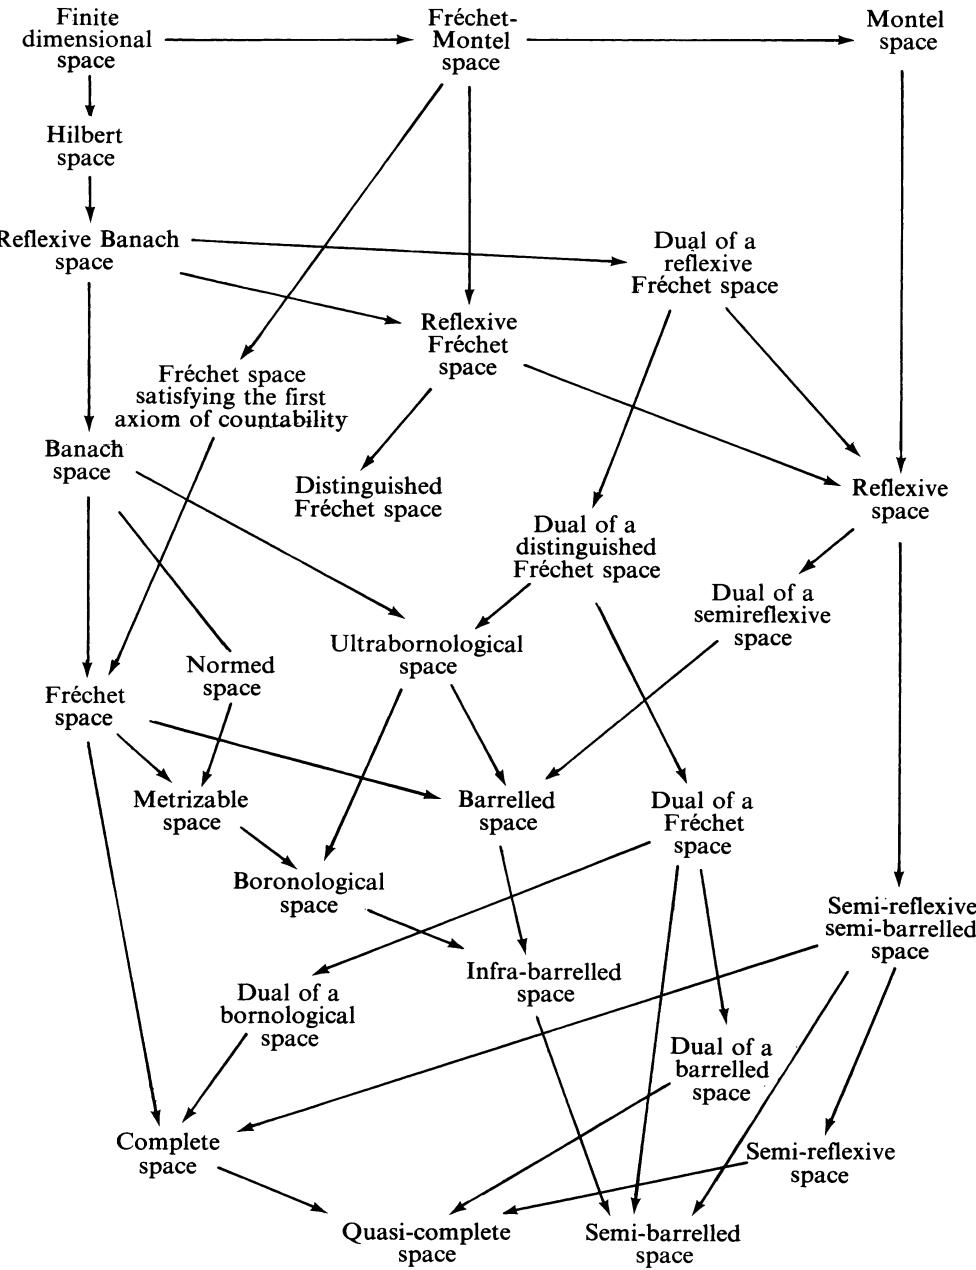
\includegraphics[keepaspectratio]{images/part002_27b26067.jpg}}

\bourbakitable{Principal bornologies on the dual of a locally convex space}{}
\pandocbounded{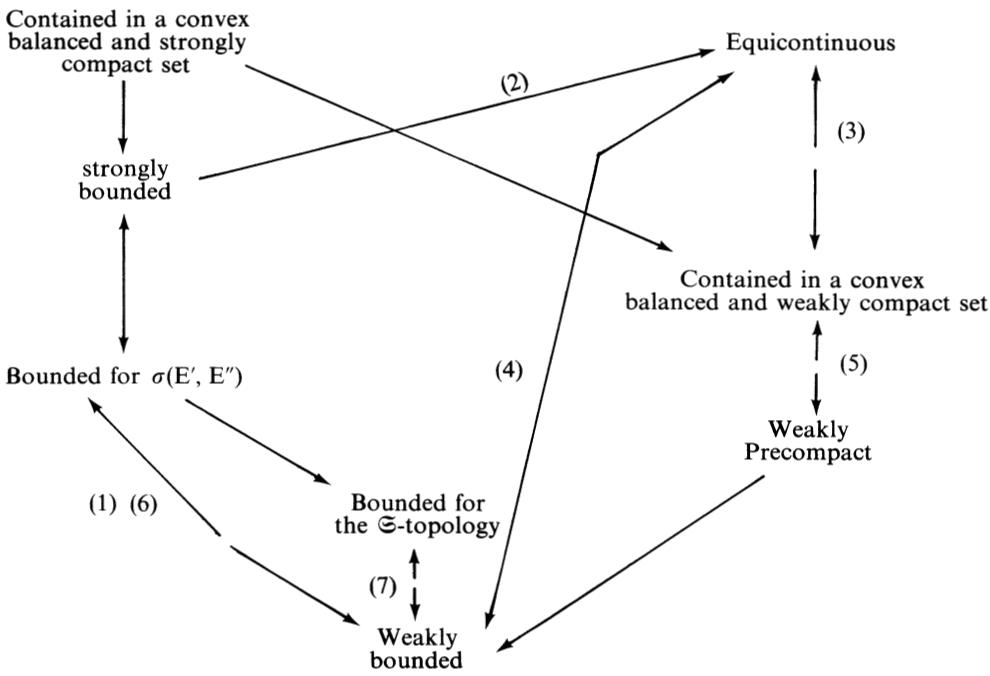
\includegraphics[keepaspectratio]{images/part002_d08e803b.jpg}}

N.B. --- We denote by S a family of bounded subsets of E such that every element is contained in a set belonging to S. A number on the side of an arrow indicates that the corresponding implication holds if the property with the same number is satisfied.

\paragraph{Properties}

\begin{enumerate}
\def\labelenumi{\arabic{enumi})}
\item
  Whenever E is semi-reflexive;
\item
  whenever E is bornological (III, p.~22, prop. 10);
\item
  if and only if E has the Mackey topology \(\tau(\mathrm{E},\mathrm{E}^{\prime})\) ;
\item
  if and only if E is barrelled;
\item
  if and only if \(\mathbf{E}'\) is quasi-complete for \(\sigma (\mathbf{E}',\mathbf{E})\)
\item
  whenever E is semi-complete (a fortiori, quasi-complete or complete) (III, p.~27, cor. 1);
\item
  whenever \(\mathfrak{S}\) consists of sets whose closed convex balanced envelope is semi-complete (III, p.~27, th. 2).
\end{enumerate}

When E is a Montel space, all the preceding bornologies are identical.

